%%%%%%%%%%%%%%%%%%%%%%%%%%%%%%%%%%%%%%%%%%%%%%%%%%%%%%%%%%%%%%%%%%%%%%%%%%%
%%%%%%%%		 Proyecto Fin de Carrera		   %%%%%%%%
%%%%%%%%	       Presentación de diapositivas		   %%%%%%%%
%%%%%%%%%%%%%%%%%%%%%%%%%%%%%%%%%%%%%%%%%%%%%%%%%%%%%%%%%%%%%%%%%%%%%%%%%%%

\documentclass[utf8, compress]			{beamer}

%%%%%%%%%%%%%%%%%%%%%%%%%        Preámbulo        %%%%%%%%%%%%%%%%%%%%%%%%%

%---------------------------------beamer----------------------------------%

\mode<presentation>
{
    \useinnertheme{rounded}
    \useoutertheme[subsection=true]{miniframes}
    \useoutertheme{split}
    \useoutertheme{shadow}
    \setbeamertemplate{headline}[miniframes theme]{}
    \defbeamertemplate{footline}{pfc slides footline}{
	\leavevmode %
	\hbox{\begin{beamercolorbox} %
	    [wd		= .58\paperwidth, %
	     ht		= 2.5ex, %
	     dp		= 1.125ex, %
	     leftskip	= .3cm plus1fill, %
	     rightskip	= .3cm]{author in head/foot} %
	    \usebeamerfont{author in head/foot}\insertshorttitle
	  \end{beamercolorbox} %
	  \begin{beamercolorbox} %
	    [wd		= .38\paperwidth, %
	     ht		= 2.5ex, %
	     dp		= 1.125ex, %
	     leftskip	= .3cm, %
	     rightskip	= .3cm plus1fil]{title in head/foot} %
	    \usebeamerfont{title in head/foot}\insertshortinstitute
	  \end{beamercolorbox}} %
    	\vskip0pt %
    }
    \setbeamertemplate{footline}[pfc slides footline]{}
    \setbeamertemplate{frametitle}[shadow theme]{}
    \setbeamertemplate{itemize items}[circle]{}
    \setbeamertemplate{enumerate items}[circle]{}
    \setbeamerfont{itemize/enumerate subbody}{size=\normalsize}
    \setbeamerfont{itemize/enumerate subsubbody}{size=\small}
    \setbeamertemplate{sections/subsections in toc}[circle]{}
    \setbeamertemplate{title page}{
	\vbox{}
	\vfill
	\begin{center}
	    \begin{beamercolorbox}[sep=8pt,center]{institute}
		\usebeamerfont{author}\insertinstitute
	    \end{beamercolorbox}
	    \inserttitlegraphic
	    \vskip.4em\par
	    \begin{beamercolorbox}[sep=8pt,center,rounded=true]{title}
		\usebeamerfont{title}\inserttitle
	    \end{beamercolorbox}
	    \vskip.4em\par
	    \begin{beamercolorbox}[sep=8pt,center]{date}
		\usebeamerfont{date}\insertdate
	    \end{beamercolorbox}
	    \begin{beamercolorbox}[sep=8pt,right]{author}
		\usebeamerfont{institute}\insertauthor
	    \end{beamercolorbox}
	\end{center}
	\vfill
    }
    \usecolortheme{orchid}
    \usecolortheme{whale}
}

%--------------------------------\beamer----------------------------------%

\usepackage[spanish]					{babel}
\usepackage[T1]						{fontenc}
\usepackage[altbullet, nofontinfo]			{lucidabr}
\usepackage						{graphicx}
\usepackage{array, booktabs, listings, multimedia}


%--------------------------------listings---------------------------------%
\lstloadlanguages{Matlab}

\lstset{language      = Matlab,
	basicstyle    = \ttfamily,
	keywordstyle  = \sffamily\bfseries,
	extendedchars = true,
	breaklines,
	captionpos    = b,
	morekeywords  = {addchannel,     analoginput, catch,
	datadqcallback,	 daqfind,        daqhwinfo,   errordlg,
	gcbo,            getdata,        guidata,     localDaqCallback,
	peekdata,        single_channel, start,       stop,
	strcmpi,	 trigger,        try,         warning}
}

\lstdefinestyle{displayed}{
	float            = tpbh,           tabsize     = 5,
	abovecaptionskip = \bigskipamount, gobble      = 4,
	xleftmargin      = .082\textwidth, numbers     = left,
	numberstyle      = \tiny,          numbersep   = 5pt
}
%-------------------------------\listings---------------------------------%

\graphicspath{{./pictures/}{../pictures/}}			% graphics

\title[ENDUS: Sistema de medida y aplicación en palmeras in vivo.]{
    Desarrollo de sistema de medida por ultrasonidos de baja frecuencia. \\
    Aplicación al análisis de palmeras in vivo.
}

\newlength{\director}
\settowidth\director{\usebeamerfont{institute}DIRECTOR: Alberto Rodríguez
    Martínez}

\author[José Ramón Gisbert Valls]{
    \vbox{
	\makebox[\director][r]{AUTOR: José Ramón Gisbert Valls}
	\makebox[\director][r]{DIRECTOR: Alberto Rodríguez Martínez}
    }
}

\institute[Universidad Miguel Hernández de Elche]{
    Universidad Miguel Hernández de Elche \medskip\par
    Escuela Politécnica Superior de Elche
}

\date[Septiembre --- 2011]{
    Proyecto Fin de Carrera \\
    Septiembre --- 2011
}

\titlegraphic{
    
\includegraphics[viewport = 0 524 152 678, clip, height = 1.4cm,
	keepaspectratio]{logo.pdf}
}

\logo{
    
\includegraphics[viewport = 0 524 152 678, clip, height = .8cm,
	keepaspectratio]{logo.pdf}
}

% Convenios tipográficos: siglas (primera vez), siglas, funciones,
% argumentos, propiedades, atributos de propiedades, nombres de canal o
% puerto
\newcommand\psig[1]{\emph{\MakeTextUppercase{#1}}}
\newcommand\sig [1]{\textsc{\MakeTextLowercase{#1}}}
\newcommand\func[1]{\texttt{#1}}
\newcommand\argu[1]{\texttt{#1}}
\newcommand\prop[1]{\textsf{#1}}
\newcommand\atr [1]{\textsf{#1}}
\newcommand\can [1]{\sig{#1}}

% Palabras predefinidas
\newcommand\matlab{\sig{MATLAB}}
\newcommand\kpci  {\sig{KPCI}-3108}
\newcommand\datx  {\sig{DAT}}
\newcommand\gui   {\sig{GUI}}
\newcommand\guide {\sig{GUIDE}}
\newcommand\pc    {\sig{pc}}
\newcommand\ram   {\sig{ram}}
\newcommand\AOUA  {\ensuremath{\mu}\sig{a}741}
\newcommand\kms   {kmus/s}

%%%%%%%%%%%%%%%%%%%%%%%%         Contenido         %%%%%%%%%%%%%%%%%%%%%%%%

\begin{document}


\frame[plain]{\titlepage}

\begin{frame}{Objetivos}
    \begin{enumerate}
	\item Desarrollo de un \alert{sistema de medida por
	    ultrasonidos}.
	    \begin{itemize}
		\item Información visual de la señal.
		\item Señal y espectro digitalizados.
	    \end{itemize}
	\item Realización de un estudio preliminar utilizando
	    \alert{ENDUS en palmeras}.
	    \begin{itemize}
		\item Relación entre los parámetros medidos y las propiedades
		    del material.
		\item Justificar un estudio posterior.
	    \end{itemize}
    \end{enumerate}
\end{frame}


\section{Desarrollo del sistema de medida}

\begin{frame}{Índice}
    \tableofcontents[currentsection]
\end{frame}


\subsection{Subsistema físico}

\begin{frame}{Transductores y acondicionadores}
    \begin{itemize}
	\item Transductores generadores (efecto piezoeléctrico).
	\item Acondicionamiento del actuador:
	    \begin{itemize}
		\item Máxima potencia transmitida.
		\item Frecuencia de oscilación de 40 kHz.
		\item Señal pulsada.
	    \end{itemize}
	\item Acondicionamiento del sensor:
	    \begin{itemize}
		\item Adaptación de impedancias.
		\item Ganancia elevada.
		\item Ancho de banda.
	    \end{itemize}
    \end{itemize}
\end{frame}


\subsection{Subsistema de adquisición}

\begin{frame}{Tarjeta de adquisición digital}
    \alert{figura}
\end{frame}

\begin{frame}{Características de la tarjeta}
    \begin{itemize}
	\item Subsistema hardware de adquisición de señales analógicas.
	    \begin{itemize}
		\item Rendimiento máximo de muestreo de 100 kmus/s.
		\item 16 canales de entrada analógica configurables por software.
		\item Amplificador de instrumentación implementado internamente en
		    la tarjeta, ganancia configurable por software.
		\item Conversor A/D de 16 bits de precisión.
		\item Cola de muestreo de 256 posiciones.
		\item Buffer FIFO con capacidad para 2048 muestras.
	    \end{itemize}
    \end{itemize}
\end{frame}

\begin{frame}{Caja de conexiones (vista externa)}
    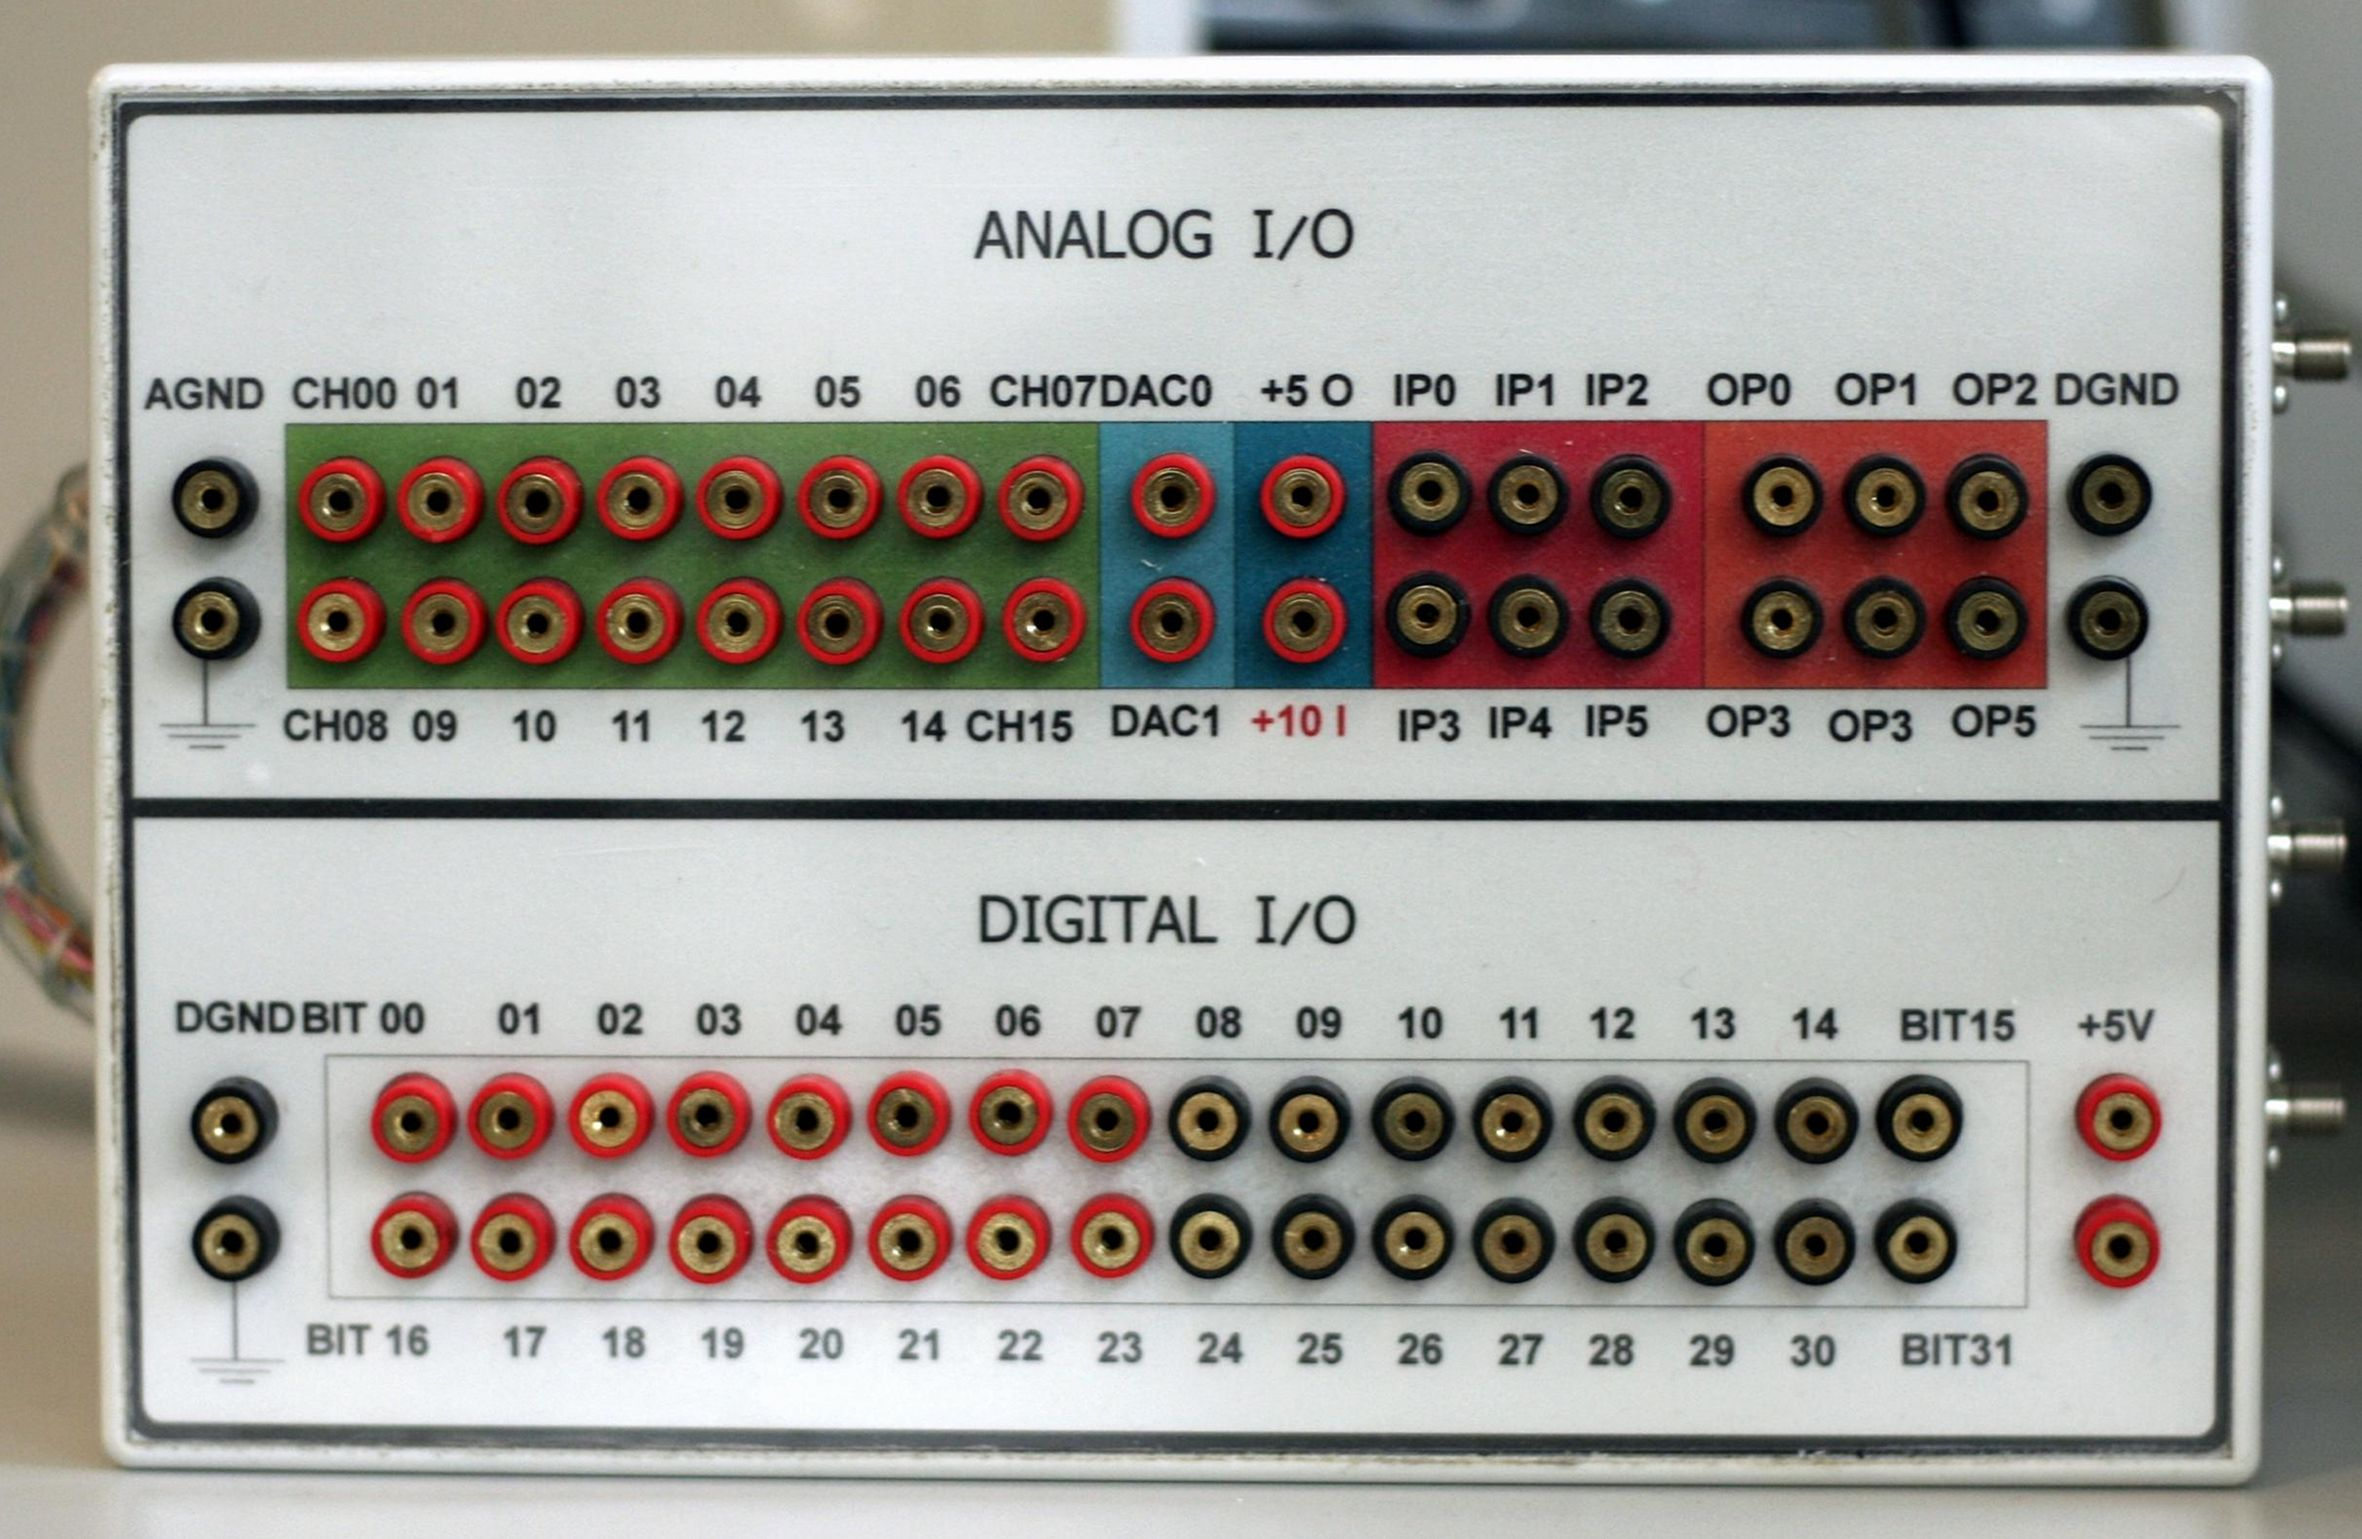
\includegraphics{exterior.jpg}
\end{frame}

\begin{frame}{Caja de conexiones (vista interna)}
    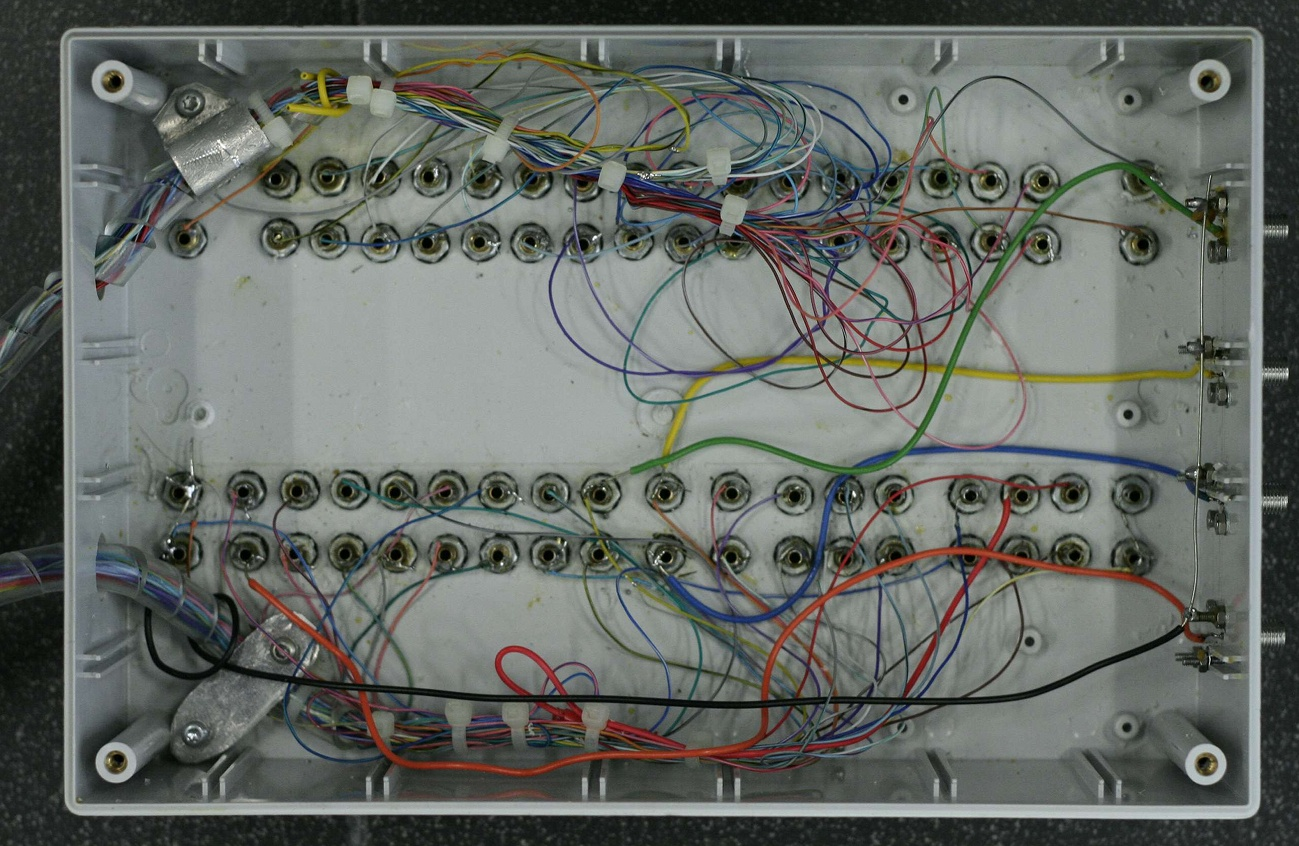
\includegraphics{interior.jpg}
\end{frame}


\subsection{Subsistema de control y presentación}

\begin{frame}{Programación de la aplicación}
    \begin{enumerate}
	\item Determinar los objetivos de programación.
	    \begin{itemize}
		\item Valor numérico instantáneo de la señal.
		\item Media aritmética de las muestras tomadas durante un
		    periodo de 250 ms.
		\item Representación gráfica de la señal.
		\item Representación gráfica del espectro instantáneo de la
		    señal.
	    \end{itemize}
	\item Aprendizaje para la utilización del SDK.
	\item Observación del modelo.
	\item Proceso de programación.
    \end{enumerate}
\end{frame}


\subsection{Conclusiones y futuras líneas de trabajo}

\begin{frame}{Índice}
    \tableofcontents[currentsubsection]
\end{frame}

\begin{frame}{Prestaciones del sistema}
    \begin{center}
	\movie[showcontrols=true, height=55mm, width=73.33mm]
	    {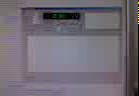
\includegraphics[height=55mm, width=73.33mm]{poster.png}}
	    {proyecto.mov}
    \end{center}
\end{frame}

\begin{frame}{Futuras líneas de trabajo}
    \begin{itemize}
	\item Limitación del sistema en frecuencia.
	\item Limitación de los transductores en potencia.
	\item Añadir nuevas funcionalidades a la aplicación.
    \end{itemize}
\end{frame}


\section{Estudio preliminar de la madera de palmera}

\begin{frame}{Índice}
    \tableofcontents[currentsection]
\end{frame}


\subsection{Teoría de los ENDUS}

\begin{frame}{Características de los ultrasonidos}
    \begin{itemize}
	\item Son perturbaciones mecánicas que viajan a través de un medio
	    elástico.
	\item Banda de frecuencia de 20 kHz a 1000 MHz (límite
	    tecnológico).
	\item Banda de frecuencia utilizada en ENDUS de 20 kHz a 25~MHz.
	\item Sus propiedades son invariantes con la frecuencia.
	\item Cuatro tipos de onda ultrasónica: longitudinales,
	    transversales, de superficie y ondas de Lamb.
    \end{itemize}
\end{frame}

% Particularidades de los ENDUS
\begin{frame}{Ensayos no destructivos por ultrasonidos}
    \begin{itemize}
	\item Campo generado por un transductor cilíndrico, resolución de
	    un ensayo.
	\item Técnicas de transmisión y de pulso"=eco.
	\item Dispersión y ruido estructural o de grano.
	\item Técnicas de postprocesado destinadas a eliminar el ruido
	    estructural.
    \end{itemize}
\end{frame}


\subsection{Estudio preliminar de la madera de palmera}

\begin{frame}{Objetivos del estudio}
    \begin{itemize}
	\item Interés en determinar las características del material.
	\item Pocas referencias que documenten la realización de ENDUS en
	    madera.
	\item Peculiaridades de la madera de palmera.
	\item Disponibilidad de unos transductores de impacto
	\item \alert{Sentar unas bases para la realización de estudios
	    posteriores.}
    \end{itemize}
\end{frame}

\begin{frame}{Peculiaridades de la madera de palmera}
    \alert{figura}
\end{frame}

\begin{frame}{Metodología}
    \alert{figura} 
\end{frame}

\begin{frame}{Metodología}
    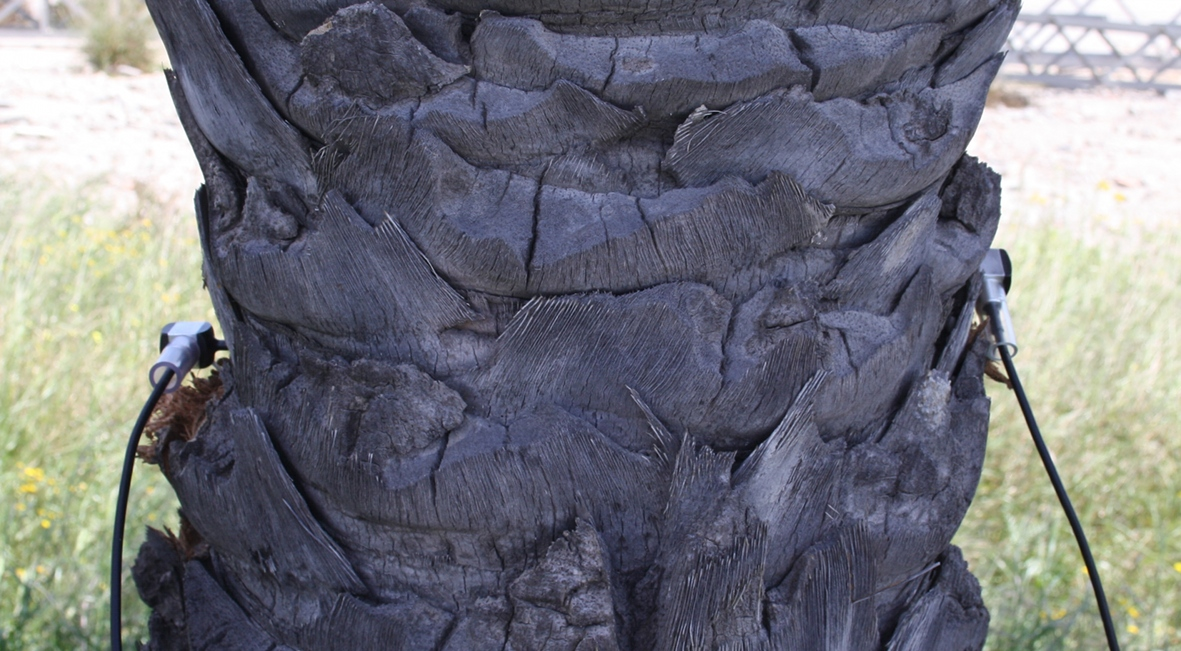
\includegraphics{mpalmera.jpg}
    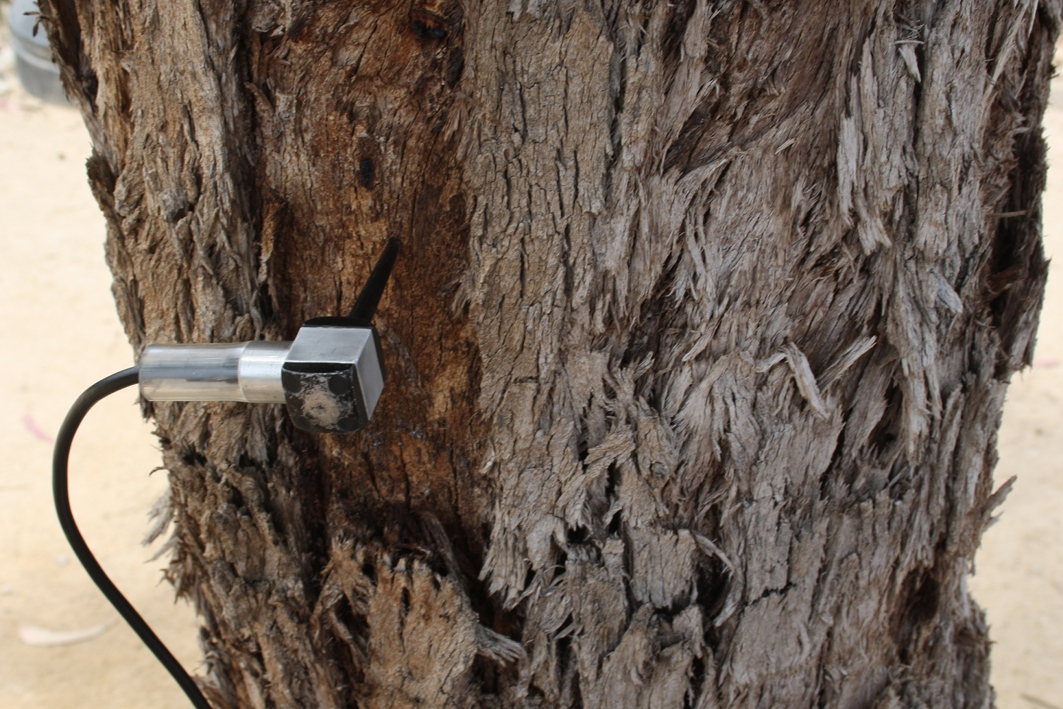
\includegraphics{meucalipto.jpg}
\end{frame}


\subsection{Conclusiones y futuras líneas de trabajo}

\begin{frame}{Índice}
    \tableofcontents[currentsubsection]
\end{frame}

\begin{frame}{Resultados de los ensayos}
    \begin{figure}
	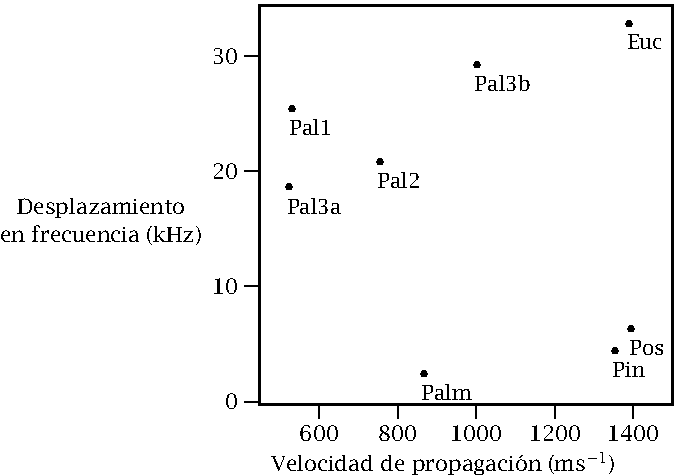
\includegraphics[height=55mm, keepaspectratio]{resultados.pdf}
	\caption{Resultados obtenidos en las pruebas}
	\label{fig:results}
    \end{figure}
\end{frame}

\begin{frame}{Futuras líneas de trabajo}
    \begin{itemize}
	\item Se recomienda un profundo estudio teórico y la
	    realización de más ensayos para determinar que relación
	    existen entre los resultados de un ENDUS y el estado
	    del ejemplar.
    \end{itemize}
\end{frame}


\end{document}
